%TODO: Latex Zeilenumbrüche korrigieren
Die Übertragungsfunktion ist die Systembeschreibung im Laplace-Bereich.\\
Sie berücksichtigt die Anfangswerte nicht. Sie geht aus der E/A-Differential\-gleichung hervor, wobei die Anfangswerte auf Null gesetzt werden. Folglich hat sie eine geringere Aussagekraft, als die E/A-Differentialgleichung, bei der die Anfangswerte immer mit dabei stehen. Es ist ein Leichtes aus der Übertragungsfunktion auf die E/A-Differentialgleichung zu schließen.
% Durch Überkreuzmultiplikation von $G(s)=\frac{Y(s)}{U(s)}=(...)$ gelangt man zu $(...)Y(s)=(...)U(s)$ und unter Beachtung von $s=\frac{d}{dt}$ zu $\ddot{y}+y=\dot{u}+u$ mit $y(0_{-})=y_{0}$, $y(0_{-})=\dot{y}_{0}$ und $u(0_{-})=u_{0}$. %TODO: ????
\subsection{Parametrische Darstellung} %TODO
%CHRIS:
Die Parametrische Darstellung erhält man, indem man die Laplace-Rücktransformierte der Übertragungsfunktion bildet.
Das macht man wie folgt:\\
Die Symbolic Toolbox macht die Ausführung symbolischer mathematischer Berechnungen möglich.\\
Mit dem Befehl\\
\texttt{syms s t}\\
erstelle ich mir eine symbolische Variable s und t.\\
Mit\\
\texttt{G(s)=(-25)/(10*s+1)}\\
gebe ich die Übertragungsfunktion G(s) ein.

Alternativ kann ich die Sprungantwort h(t) durch Integration der Übertragungsfunktion bestimmen, gebe ich den Befehl \\
\texttt{ilaplace(G(s)/s)}\\
ein.

%ICH:
%ilaplace(G(s)/s), alternativ kann h(t) auch durch Integration von G(t) berechnet werden. h(t)=int(g(t))
%Möchte ich mein Ergebnis g(t) weiter verwenden und nicht ans benutzen, dann definiere ich mir die symbolische Funktion syms g(t)

%Alternativ kann die Übergangsfunktion aus der Gewichtsfunktion durch Integration erhalten werden.

Diese Sprungantwort wäre dann:
\begin{equation*}
    h(t)=25*e^{\frac{-t}{10}}-25
\end{equation*}

Hier graphisch dargestellt:
\begin{figure}[H]
    \centering
    \includegraphics[width=5cm]{image/Übergangsfunktion.eps}
    \caption{Übergangsfunktion $h(t)$}
\end{figure}


\subsection{Nichtparametrische Darstellung}
\subsubsection{Plot mit Matlab}

Mit dem Wissen der Parametrischen Darstellung\\ 
\texttt{t=[0:0.1:10]}\\
\texttt{plot(t, (25)*exp(-t/10)-25)}\\
Da t ein Vektor ist, muss man beim Multiplizieren das Punktprodukt (Hadammad-Produkt) verwenden.

        
%Die Control System Toolbox dient der systematischen Analyse, dem Entwurf und der Optimierung linearer Systeme.\\
%Mit dem folgenden Matlab-Skript kann ich die Übertragungsfunktion G(s) in MATLAB eingeben.
%\lstinputlisting[style=Matlab-editor, caption={pretty}]{../MATLAB/ControlSystemToolbox/cst_DTs.m}
%Lässt man sich G(s) in der Konsole anzeigen, wird diese folgendermaßen dargestellt.
                    
%Durch den Befehl \texttt{step(sys)} öffnet MATLAB ein neues Fenster mit der passenden Sprungantwort h(s) zu G(s) und stellt diese folgendermaßen dar.
\begin{figure}[H]
    \centering
    \includegraphics[width=5cm]{image/PlotMitMatLab.eps}
    \caption{Sprungantwort Plot mit Matlab}
\end{figure}
\subsubsection{Plot mit Step-Funktion}
Denselben Plot bekommt
\subsubsection{Plot mit Simulink}
...